\chapter{Verification with Mathematica}
\section{Simple Pendulum}
Mathematica was used to verify some of the results generated by the programs written.
To verify that the algorithm was implemented correctly Mathematica was used to
solve the system of differential equations for a pendulum using Mathematica's
internal differential equation solving algorithms. A pendulum with a length of
1, mass of 1 and a force of -1 in the y direction was setup. The 
graphs of the x and y position of the particle are shown in figure
\ref{Fig:x_single_pendulum} and figure \ref{Fig:y_single_pendulum}.

\begin{figure} 
	\begin{center}
		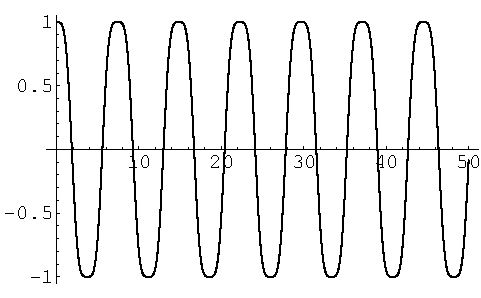
\epsfig{file=./x_single_pendulum.pdf}
	\end{center}
    \caption{x value vs time (derived using Mathematica)}
\label{Fig:x_single_pendulum}   
\end{figure}
\begin{figure}    
	\begin{center}
		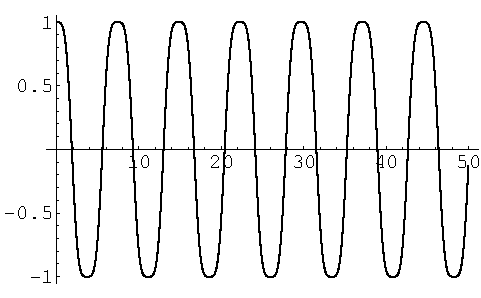
\epsfig{file=./x_single_pendulum_simple_constr.pdf}
	\end{center}
    \caption{x value vs time using simple constraint based dynamics}
	\label{Fig:x_single_pendulum_simple_constr}
\end{figure}  

Subsequently an implementation of a pendulum using the constraint formulation
given in \ref{Eqn:LambdaSimple} was implemented in C++. The numerical
integration technique used was RK4. The behaviour of the particle was expected
to be similar to the solution derived using Mathematica, and therefore the
graphs should look similar. It was not expected that the exact numerical values
be the same since Mathematica uses a more sophisticated algorithm to numerically
solve the differential equations than the RK4 solver implemented for this
thesis.  The graphs of the x and y positions are shown in figures
\ref{Fig:x_single_pendulum_simple_constr} and
\ref{Fig:y_single_pendulum_simple_constr}.

\begin{figure}    
	\begin{center}
		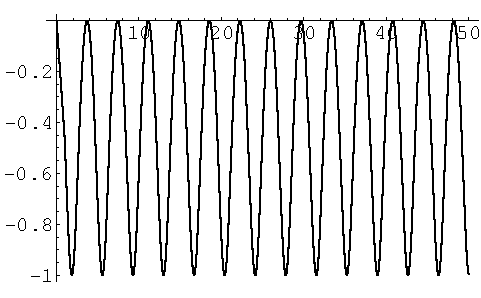
\epsfig{file=./y_single_pendulum.pdf}
	\end{center}
    \caption{y value vs time (derived using Mathematica)}
	\label{Fig:y_single_pendulum}
\end{figure}
\begin{figure}    
	\begin{center}
		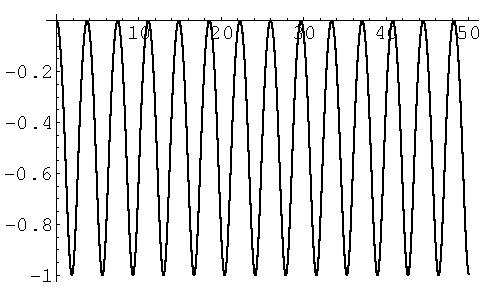
\epsfig{file=./y_single_pendulum_simple_constr.pdf}
	\end{center}
    \caption{y value vs time using simple constraint based dynamics}
	\label{Fig:y_single_pendulum_simple_constr}
\end{figure} 

\section{Double Pendulum}
In order to verify that the generic constraints were working working in a
plausable manner a double pendulum system was implemented in three different
ways. The first way used Mathematica to solve the equations of motion using
Newtonian methods. The set of differential equations for $\Theta_1$ and
$\Theta_2$ (see \footnote{\url{http://www.myphysicslab.com/}}) was given to
Mathematica and a solution found using Mathematica's default solver. Mathematica
was employed again to solve the system using a Lagrangian formulation of the
double pendulum system.  Unexpectedly the solution was slightly different
depending on the technique used (i.e.  Newtonian or Lagrangian). Evidence of
this is shown in the graphs \ref{Fig:x1_newtonian}, \ref{Fig:x1_lagrangian}, 
\ref{Fig:y1_newtonian} and \ref{Fig:y1_lagrangian}. The graphs show the movement of a double
pendulum over time, initially set with both angles at $\frac{\Pi}{8}$.

\begin{figure}
	\begin{center}
		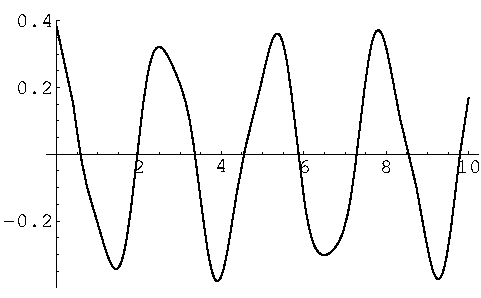
\epsfig{file=./x1_newtonian.pdf}
	\end{center}
    \caption{\label{Fig:x1_newtonian}x position of the 1st particle obtained using Newtonian methods}
	\begin{center}
		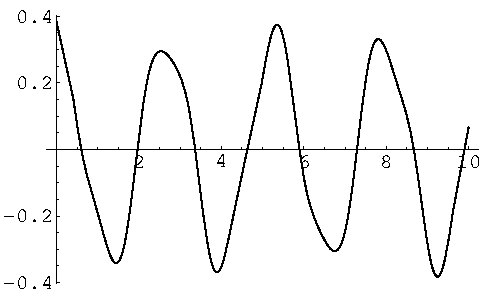
\epsfig{file=./x1_lagrangian.pdf}
	\end{center}
    \caption{\label{Fig:x1_lagrangian}x position of the 1st particle obtained using Lagrangian methods}
\end{figure}

\begin{figure}
	\begin{center}
		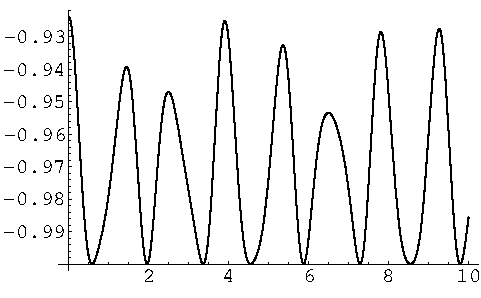
\epsfig{file=./y1_newtonian.pdf}
	\end{center}
    \caption{\label{Fig:y1_newtonian}y position of the 1st particle obtained using Newtonian methods}
	\begin{center}
		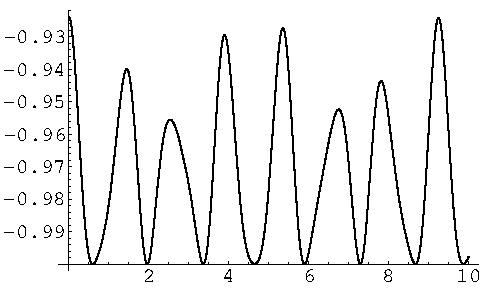
\epsfig{file=./y1_lagrangian.pdf}
	\end{center}
    \caption{\label{Fig:y1_lagrangian}y position of the 1st particle obtained using Lagrangian methods}
\end{figure}

Finally the third method employed two fixed distance constraints and one fixed
position constraint. The matrix equation \ref{Eqn:LambdaStable} was solved using
a biconjugate gradient solver \cite{NumRecipes} and the resulting differential
system solved using a Runga-Kutta 4 implementaion. The graphs of the motion of
the particle are shown in figures \ref{Fig:x1_constr_double_pendulum},
\ref{Fig:x1_double_pendulum}, \ref{Fig:y1_constr_double_pendulum} and
\ref{Fig:y1_double_pendulum}.  It was expected that the motion of the particles
be similar, but not exactly the same since the double pendulum is a chaotic
system. However, the graphs illustrate disconcerting differences between the
constrained dynamics implementation and the graph derived using Mathematica.

\begin{figure}
	\begin{center}
		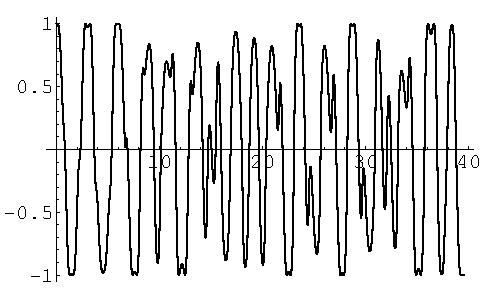
\epsfig{file=./x1_constr_double_pendulum.pdf}
	\end{center}
    \caption{\label{Fig:x1_constr_double_pendulum}x position of the 1st particle
    obtained using a constrained dynamics implementation}
	\begin{center}
		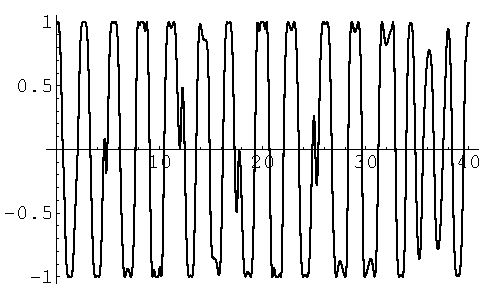
\epsfig{file=./x1_double_pendulum.pdf}
	\end{center}
    \caption{\label{Fig:x1_double_pendulum}x position of the 1st particle
    obtained using Newtonian methods and Mathematica}
\end{figure}

\begin{figure}
	\begin{center}
		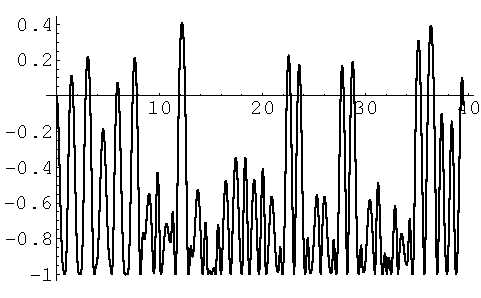
\epsfig{file=./y1_constr_double_pendulum.pdf}
	\end{center}
    \caption{\label{Fig:y1_constr_double_pendulum}y position of the 1st particle
    obtained using a constrained dynamics implementation}
	\begin{center}
		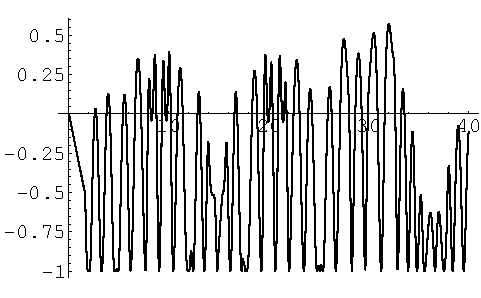
\epsfig{file=./y1_double_pendulum.pdf}
	\end{center}
    \caption{\label{Fig:y1_double_pendulum}y position of the 1st particle
    obtained using Newtonian methods and Mathematica}
\end{figure}

